%%%%%%%%%%%%%%%%%%%%%%%%%%%%%%%%%%%%%%%%%%%%%%%%%%%%%%%%%%%%%%%%%%%%
%% I, the copyright holder of this work, release this work into the
%% public domain. This applies worldwide. In some countries this may
%% not be legally possible; if so: I grant anyone the right to use
%% this work for any purpose, without any conditions, unless such
%% conditions are required by law.
%%%%%%%%%%%%%%%%%%%%%%%%%%%%%%%%%%%%%%%%%%%%%%%%%%%%%%%%%%%%%%%%%%%%

\documentclass{beamer}
\usetheme[faculty=fi]{fibeamer}
%\usepackage[utf8]{inputenc}
\usepackage[T1]{fontenc}
\def\TextUnderscore{\char\`_} 
\usepackage[
  main=czech, %% By using `czech` or `slovak` as the main locale
                %% instead of `english`, you can typeset the
                %% presentation in either Czech or Slovak,
                %% respectively.
  english, slovak %% The additional keys allow foreign texts to be
]{babel}        %% typeset as follows:
%%
%%   \begin{otherlanguage}{czech}   ... \end{otherlanguage}
%%   \begin{otherlanguage}{slovak}  ... \end{otherlanguage}
%%
%% These macros specify information about the presentation
\title{Používání a získávání kryptoměny Monero z pohledu použitelné bezpečnosti} %% that will be typeset on the

\subtitle{21. června 2019} %% title page.
\author{Bc. Radim Lipovčan, 433279@muni.cz}
%% These additional packages are used within the document:
\usepackage{ragged2e}  % `\justifying` text
\usepackage{booktabs}  % Tables
\usepackage{tabularx}
\usepackage{tikz}      % Diagrams
\usetikzlibrary{calc, shapes, backgrounds}
\usepackage{amsmath, amssymb}
\usepackage{url}       % `\url`s
\usepackage{listings}  % Code listings
\frenchspacing

\usepackage{graphicx}
\graphicspath{ {./resources/} }
\usepackage{multicol}


\usepackage{pgfplots}
\def\angle{0}
\def\radius{3}
\def\cyclelist{{"orange","blue","red","green"}}
\newcount\cyclecount \cyclecount=-1
\newcount\ind \ind=-1
%\usepackage{pgf-pie}
\usepackage{anyfontsize}

%plots
\usepackage{tikz,fourier,ifthen}

\colorlet{color0}{blue!40}
\colorlet{color1}{orange!60}
\colorlet{color2}{green!60}
\colorlet{color3}{yellow!60}
\colorlet{color4}{red!60}
\colorlet{color5}{blue!60!cyan!60}
\colorlet{color6}{cyan!60!yellow!60}
\colorlet{color7}{red!60!cyan!60}
\colorlet{color8}{red!60!blue!60}
\colorlet{color9}{orange!60!cyan!60}





%beginchartstacked
\newlength{\xdim}

\definecolor{1}{HTML}{00A64F}
\definecolor{2}{HTML}{8DC73E}
\definecolor{3}{HTML}{974006}
\definecolor{4}{HTML}{F58137}
\definecolor{5}{HTML}{ED1B23}
\definecolor{6}{HTML}{949698}
\definecolor{7}{HTML}{911118}

%endchartstacked

%branches
\usepackage{tikz}
%
\usetikzlibrary{trees}

%flowchart
\usetikzlibrary{shapes,arrows}
\usetikzlibrary{positioning}

%ringct
\usetikzlibrary{arrows,shapes,snakes,automata,backgrounds,petri}

%code
\renewcommand{\texttt}[1]{%
  \begingroup
  \ttfamily
  \begingroup\lccode`~=`/\lowercase{\endgroup\def~}{/\discretionary{}{}{}}%
  \begingroup\lccode`~=`[\lowercase{\endgroup\def~}{[\discretionary{}{}{}}%
  \begingroup\lccode`~=`.\lowercase{\endgroup\def~}{.\discretionary{}{}{}}%
  \catcode`/=\active\catcode`[=\active\catcode`.=\active
  \scantokens{#1\noexpand}%
  \endgroup
}
\usepackage{dirtytalk}
\begin{document}

  \frame{\maketitle}

  \AtBeginSection[]{% Print an outline at the beginning of sections
    \begin{frame}<beamer>
      \frametitle{Obsah sekce \thesection}
		\begin{multicols}{2}      
      \tableofcontents[currentsection]
      \end{multicols}
    \end{frame}}

  \begin{darkframes}
    \section{Motivace}
    \subsection{SSME}
    \begin{frame}{Motivace | SSME}
    Při výběru tématu bylo potřeba dbát pozor na:
		\begin{itemize}
		\item Důraz na T-shape, jak jej zohlednit v diplomové práci?
		\item "Diplomová práce by měla reflektovat tvůj Interim Projekt nebo alespoň zkušenosti v něm nabyté." \begin{itemize}
		\item převzato z http://ssme.fi.muni.cz/student/studium)
		\end{itemize}
		\end{itemize}		     
     
	    \end{frame}
    \subsection{Monero}
    \begin{frame}{Motivace | Monero}
		\begin{itemize}
		\item Open-source kryptoměna
    	\item Zaměření na anonymitu, decentralizaci
     	\item Aktivní komunita na GitHubu a na Redditu včetně dalších sociálních sítí
		\end{itemize}  
		\begin{figure}
  \centering
  
\includegraphics[width=1\textwidth]{monero-github.png}
  
\includegraphics[width=0.4\textwidth]{monero-reddit.png}
  \caption{Monero Github \& Reddit.}  \label{fig:xray}
\end{figure}
		  
    \end{frame}
    \subsection{Cíl diplomové práce}
    \begin{frame}{Motivace | Cíl diplomové práce}
     Zkombinovat:
     \begin{itemize}
     \item Znalosti nabyté na intermu, studiu, rozsah T-shape
     \item Technické téma kryptoměny Monero
     \end{itemize}
     	Cílem:
		\begin{itemize}
		\item Zmapovat způsoby získávání a užívání kryptoměny Monero
		\item Uživatelská část - využití kryptoměny
		\item Těžební část - software, pooly, systémy pro těžbu
		\item Obě části - provést výzkum na dané části komunity
		\begin{itemize}
		\item A vytěžit z toho nové věci - best practices + automatizace
		\end{itemize}
		\end{itemize}
    \end{frame}
  \end{darkframes}

  \AtBeginSection[]{% Print an outline at the beginning of sections
    \begin{frame}<beamer>
      \frametitle{Obsah sekce \thesection}
      \begin{multicols}{2}      
      \tableofcontents[currentsection]
      \end{multicols}
    \end{frame}}
    
  \begin{darkframes}
    \section{Kryptoměna Monero}
    \subsection{Informace o krypoměně}
    \begin{frame}{Kryptoměna Monero | Informace o krypoměně}
    Open-source kryptoměna vyvíjená pod Monero projektem.
    Cílem je mít decentralizovanou a anonymní kryptoměnu.
    
\begin{itemize}[<+->]
\item<1-4>  Žádnou transakci nelze jednoduše vysledovat zpátky k uživateli a ani nelze zjistit kolik Monera bylo posláno.
\item<2-4> Použití CryptoNote protokolu.
\item<3-4> Blockchain je veřejný, většina je šifrovaná.
\item<4-4> Pro anonymitu krpytoměny jsou použity technologie: 
\begin{itemize}
\item Ring Signatures (skrytí odesílatele)
\item RingCT (skrytí posílané částky)
\item Stealth Addresses (skrytí příjemce a historie transakce)
\end{itemize}
\end{itemize}    

     \begin{figure}
  
\includegraphics[width=0.2\textwidth]{monero-icon.png}
  \caption{Monero Github \& Reddit.}  \label{fig:xray}
\end{figure}
    \end{frame}
    \subsection{Popis systému}
    \begin{frame}{Kryptoměna Monero | Popis systému}
   Před samotným výzkumem a tvorbou:
     \begin{itemize}[<+->]
     \item<1-3> Vývojový cyklus
     \item<1-3> Princip transakcí
     \item<2-3> Fungování peněženek
     \item<2-3> Útoky vůči peněženkám
     \item<3-3> Problémy Monera (většinou malware)
     \item<3-3> Princip těžby
     \end{itemize}
    \end{frame}
     \begin{frame}{Kryptoměna Monero | Popis systému - ukázka transakce}
\definecolor{ao(english)}{rgb}{0.0, 0.5, 0.0}
\definecolor{azure(colorwheel)}{rgb}{0.0, 0.5, 1.0}
\definecolor{darkorange}{rgb}{1.0, 0.55, 0.0}
\tikzstyle{decision} = [diamond, draw, fill=blue!20,
    text width=4.5em, text badly centered, node distance=2.5cm, inner sep=0pt]
\tikzstyle{userA} = [rectangle, draw, fill=ao(english)!20,
    text width=5em, text centered, rounded corners, minimum height=4em]
\tikzstyle{userB} = [rectangle, draw, fill=azure(colorwheel)!20,
    text width=5em, text centered, rounded corners, minimum height=4em]
\tikzstyle{userC} = [rectangle, draw, fill=darkorange!20,
    text width=5em, text centered, rounded corners, minimum height=4em]
\tikzstyle{lineuserA} = [draw, very thick, color=ao(english)!80, -latex']

\tikzstyle{lineuserB} = [draw, very thick, color=azure(colorwheel)!80, -latex']
\tikzstyle{lineuserC} = [draw, very thick, color=darkorange!80, -latex']
\tikzstyle{cloud} = [draw, ellipse,fill=red!20, node distance=2.5cm,
    minimum height=2em]
    \resizebox{!}{200px}{\centering
\begin{tikzpicture}[scale=2, node distance = 2cm, auto,color=black]
\shorthandoff{-}
    % Place nodes
    \node [userA,text width=5cm,minimum width=5cm] (userA1) {\parbox{5cm}{\centering Transaction request generated by the client \texttt{transfer ADDRESS AMOUNT}}};
    \node [userB, right of=userA1, node distance=6cm, text width=5cm,minimum width=5cm] (userB1)    {\parbox{5cm}{\centering Request broadcast to network nodes, shown \texttt{show-transfers pool} }};
    
    \node [below of=userA1,node distance=2.5cm,text width=5cm,minimum width=5cm, draw=none] (userA2){};
    \node [userB, below of=userB1, node distance=2.5cm,text width=5cm,minimum width=5cm] (userB2)    {\parbox{5cm}{\centering Transaction is added to the block waiting to be mined.}};
    
    \node [userC, below of=userA2,node distance=2.5cm,text width=5cm,minimum width=5cm] (userA3)  {\parbox{5cm}{\centering Miners are verifying transactions in the pending block.}}; %, in cli called multisig wallet password
    \node [userB, below of=userB2, node distance=2.5cm,text width=5cm,minimum width=5cm] (userB3)    {\parbox{5cm}{\centering Every 2 minutes new Monero block is mined and added to the blockchain.}}; %, in cli called multisig wallet password
    
    
    \node [userC, below of=userA3,node distance=2.5cm,text width=5cm,minimum width=5cm] (userA4) {\parbox{5cm}{\centering Miners are rewarded by block reward.}};
    \node [userB, below of=userB3, node distance=2.5cm,text width=5cm,minimum width=5cm] (userB4)    {\parbox{5cm}{\centering Receiving party's wallet becomes aware of the transaction.}};
        
   % \node [block, below of=init, node distance=2.5cm,text width=3cm,minimum width=3cm] (identify) {\parbox{3cm}{\centering Repackaging by reseller}};
%    \node [block, below of=identify, node distance=2.5cm,text width=3cm,minimum width=3cm] (evaluate) {\parbox{3cm}{\centering HW wallet bought by enduser}};
 %   \node [cloud, left of=identify, node distance=5cm] (update) {\parbox{3cm}{\centering Malicious scratchpad with seed  }};
  %  \node [block, below of=evaluate, node distance=2.5cm,text width=3cm,minimum width=3cm] (attacker) {\parbox{3cm}{\centering Attacker's database of wallets}};
    % Draw edges
    \path [lineuserC] (userA3) -- (userB3);
   % \path [lineuserA] (userA2) -- (userA4);
    \path [lineuserB] (userB1) -- (userB2);
    \path [lineuserB] (userB2) -- (userB3);
    \path [lineuserB] (userB3) -- (userB4);
    \path [lineuserB] (userB3) to[in=14,out=210,looseness=0] (userA4);
        \path [lineuserA] (userA1) to[in=-165,out=-15,looseness=0]  (userB1);
        \path [lineuserB] (userB1) to[in=15,out=165,looseness=0]   (userA1);
   % \path [line] (identify) -- (evaluate);
   %\path [line] (expert) -- (init);
  % \path [lineuserA] (userA2) |- (userB2);
\end{tikzpicture}}
\end{frame}    
    
      \end{darkframes}


  \AtBeginSection[]{% Print an outline at the beginning of sections
    \begin{frame}<beamer>
      \frametitle{Obsah sekce \thesection}
      \begin{multicols}{2}      
      \tableofcontents[currentsection]
      \end{multicols}
    \end{frame}}
    
   
  \begin{darkframes}
    \section{Výzkum uživatelů Monera}
    \subsection{Cíl}
    \begin{frame}{Cíl výzkumu uživatelů Monera}
Zjistit informace o chování uživatelů při používání Monera a zároveň se zaměřit na práci s klíči k peněžence včetně zaměření se na samotnou bezpečnost užívání.

Dotazník rozdělen:
\begin{itemize}
\item<1-4> G01 - Introductory information
\item<1-4> G02 - Monero usage
\item<2-4> G03 - Monero key and coin management
\item<3-4> G04 - Monero and malicious things
\item<4-4> G05 - Monero recovery
\item<4-4> G06 - Special question set for miners
\item<4-4> G07 - Demographics
	\end{itemize}
	\end{frame}
    \subsection{Sběr dat}
    \begin{frame}{Sběr dat}
     \begin{itemize}
     \item 15.11.2018 - 27.01.2019
     \item LimeSurvey, na vlastním serveru
     \item Respondentům bylo doporučeno použít TOR nebo alespoň proxy
     \item CAPTCHA proti spamu a botům
     \end{itemize}
    \end{frame}
    \subsection{Výsledky}
    \begin{frame}{Výsledky | Ukázka z nasbíraných dat}
     
\begin{center}
\begin{figure}[H]
\begin{tikzpicture}
\begin{axis}[
    xbar stacked,
    y dir = reverse,
    legend style={
    legend columns=2,
        at={(xticklabel cs:0.5)},
        anchor=north,
        draw=none
    },
    ytick=data,
    axis y line*=none,
    axis x line*=bottom, %bottom
    tick label style={font=\footnotesize},
    legend style={font=\footnotesize,fill=black,draw=white},
    label style={font=\footnotesize},
    xtick={0,100},
    width=.84\textwidth,
    bar width=6mm,
    xlabel={Time in ms},
    yticklabels={Filtered responses},
    xmin=0,
    xmax=100,
    area legend,
    xticklabel={\pgfmathparse{\tick}\pgfmathprintnumber{\pgfmathresult}\%},
    y=8mm,
   % enlarge y limits={abs=0.625},
]\addplot[1,fill=1] coordinates {(62,0) };
%{(113,0) }; absolutni cisla, potrebuje to procenta
\addplot[4,fill=4] coordinates {(36,0) };
%{(67,0) };
\addplot[3,fill=3] coordinates {(1,0) };
%{(1,0) };
\addplot[6,fill=6] coordinates {(1,0) };
%{(1,0) };
\legend{Valid responses [113],Partially filled [67],Too fast response [1],Invalid [1]
}
\coordinate (A) at (30,0);% ******** start of changes ************
\coordinate (B) at (80,0);
\end{axis}  
\node at (A) {62\%};
\node at (B) {37\%};% ********* end of changes **********
\end{tikzpicture}
\caption{Celkový přehled respondentů, N=179.}
\label{chart:price}\end{figure}\end{center}
    \end{frame}
    
\begin{frame}{Výsledky | Ukázka z nasbíraných dat}
\begin{center}
\begin{figure}[H]
\begin{tikzpicture}
\begin{axis}[
    xbar stacked,
    y dir = reverse,
    legend style={
    legend columns=2,
        at={(xticklabel cs:0.5)},
        anchor=north,
        draw=none
    },
    ytick=data,
    axis y line*=none,
    axis x line*=bottom, %bottom
    tick label style={font=\footnotesize},
    legend style={font=\footnotesize,fill=black,draw=white},
    label style={font=\footnotesize},
    xtick={0,100},
    width=.83\textwidth,
    bar width=6mm,
    xlabel={Time in ms},
    yticklabels={Hot wallet, Cold wallet, View-only wallet, Exchange wallet, Web wallet, Air-gapped wallet, Paper wallet, Hardware wallet},
    xmin=0,
    xmax=100,
    area legend,
    xticklabel={\pgfmathparse{\tick}\pgfmathprintnumber{\pgfmathresult}\%},
    y=8mm,
    enlarge y limits={abs=0.625},
]
\addplot[1,fill=1] coordinates {(60,1) (44,2) (10,3) (23,4) (15,5)(7,6)(25,6)(23,7)};
\addplot[4,fill=4] coordinates {(40,1) (56,2) (90,3) (77,4) (85,5) (93,6)(75,6)(77,7)};

%{(113,0) }; absolutni cisla, potrebuje to procenta

\legend{Yes, No
}
\coordinate (A) at (50,0);% ******** start of changes ************
\coordinate (B) at (80,0);
\coordinate (C) at (20,-8mm);% ******** start of changes ************
\coordinate (D) at (75,-8mm);
\coordinate (E) at (5,-16mm);% ******** start of changes ************
\coordinate (F) at (50,-16mm);
\coordinate (G) at (12,-24mm);% ******** start of changes ************
\coordinate (H) at (50,-24mm);
\coordinate (X) at (5,-32mm);% ******** start of changes ************
\coordinate (I) at (50,-32mm);
\coordinate (J) at (12,-40mm);% ******** start of changes ************
\coordinate (K) at (50,-40mm);
\coordinate (L) at (12,-48mm);% ******** start of changes ************
\coordinate (M) at (50,-48mm);
\end{axis}  
\node at (A) {68};
\node at (B) {45}; % ********* end of changes **********
\node at (C) {49};
\node at (D) {64};% ********* end of changes **********
\node at (E) {26};
\node at (F) {87};% ********* end of changes **********
\node at (G) {11};
\node at (H) {102};% ********* end of changes **********
\node at (X) {8};
\node at (I) {105};% ********* end of changes **********
\node at (J) {17};
\node at (K) {96};% ********* end of changes **********
\node at (L) {28};
\node at (M) {85};% ********* end of changes **********
\end{tikzpicture}
\caption{Wallet types usage in Monero.}
\label{chart:monerowalletsusagechart}\end{figure}\end{center}    
        \end{frame}
   
    \begin{frame}{Výsledky | Ukázka z nasbíraných dat}
\begin{center}
\begin{figure}[H]
\begin{tikzpicture}
\begin{axis}[
    xbar stacked,
    y dir = reverse,
    legend style={
    legend columns=2,
        at={(xticklabel cs:0.5)},
        anchor=north,
        draw=none
    },
    ytick=data,
    axis y line*=none,
    axis x line*=bottom, %bottom
    tick label style={font=\footnotesize},
    legend style={font=\footnotesize,fill=black,draw=white},
    label style={font=\footnotesize},
    xtick={0,100},
    width=.82\textwidth,
    bar width=6mm,
    xlabel={Time in ms},
    yticklabels={Recovery reason},
    xmin=0,
    xmax=100,
    area legend,
    xticklabel={\pgfmathparse{\tick}\pgfmathprintnumber{\pgfmathresult}\%},
    y=8mm,
    enlarge y limits={abs=0.625},
]
\addplot[1,fill=1] coordinates {(30,1)};
\addplot[4,fill=4] coordinates {(18,1)};
\addplot[5,fill=5] coordinates {(40,1)};
\addplot[6,fill=6] coordinates {(12,1)};

%{(113,0) }; absolutni cisla, potrebuje to procenta

\legend{Disk issue, Software issue, Device error, Not specified
}
\coordinate (A) at (16,0);% ******** start of changes ************
\coordinate (B) at (40,0);
\coordinate (C) at (68,0);% ******** start of changes ************
\coordinate (D) at (94,0);
\end{axis}  
\node at (A) {15};
\node at (B) {9};% ********* end of changes **********
\node at (C) {20};
\node at (D) {6};% ********* end of changes **********
\end{tikzpicture}
\caption{Reason for wallet recovery.}
\label{chart:recoveryreason}\end{figure}\end{center}
\begin{center}
\begin{figure}[H]
\begin{tikzpicture}
\begin{axis}[
    xbar stacked,
    y dir = reverse,
    legend style={
    legend columns=3,
        at={(xticklabel cs:0.5)},
        anchor=north,
        draw=none
    },
    ytick=data,
    axis y line*=none,
    axis x line*=bottom, %bottom
    tick label style={font=\footnotesize},
    legend style={font=\footnotesize,fill=black,draw=white},
    label style={font=\footnotesize},
    xtick={0,100},
    width=.82\textwidth,
    bar width=6mm,
    xlabel={Time in ms},
    yticklabels={Restore method},
    xmin=0,
    xmax=100,
    area legend,
    xticklabel={\pgfmathparse{\tick}\pgfmathprintnumber{\pgfmathresult}\%},
    y=8mm,
    enlarge y limits={abs=0.625},
]
\addplot[1,fill=1] coordinates {(18,1)};
\addplot[2,fill=2] coordinates {(4,1)};
\addplot[4,fill=4] coordinates {(10,1)};
\addplot[5,fill=5] coordinates {(51,1)};
\addplot[6,fill=6] coordinates {(17,1)};
%{(113,0) }; absolutni cisla, potrebuje to procenta

\legend{Hard drive, Cloud storage, Flash drive, Paper media, Mnemonic seed
}
\coordinate (A) at (10,0);% ******** start of changes ************
\coordinate (B) at (20,0);
\coordinate (C) at (27,0);% ******** start of changes ************
\coordinate (D) at (55,0);
\coordinate (E) at (92,0);
\end{axis}  
\node at (A) {9};
\node at (B) {2};% ********* end of changes **********
\node at (C) {5};
\node at (D) {26};% ********* end of changes **********
\node at (E) {8};% ********* end of changes **********
\end{tikzpicture}
\caption{Method used for wallet recovery.}
\label{chart:recoverymethod}\end{figure}\end{center}    
     
    \end{frame}
    
    
    \subsection{Nejlepší praktiky}
    \begin{frame}{Nejlepší praktiky | Best practices}
     Na základě dat z průzkumu:
     \begin{itemize}
     \item Postup pro bezpečné vytvoření peněženky
     \item Návrh pro bezpečné uložení klíčů
     \item Zálohovací schéma pro klíče
     \end{itemize}
    \end{frame}
  \end{darkframes}
  
  \AtBeginSection[]{% Print an outline at the beginning of sections
    \begin{frame}<beamer>
      \frametitle{Obsah sekce \thesection}
      \begin{multicols}{2}      
      \tableofcontents[currentsection]
      \end{multicols}
    \end{frame}}
    
  \begin{darkframes}
    \section{Výzkum těžařů Monera}
    \subsection{Cíl}
    \begin{frame}{Cíl výzkumu těžařů Monera}
Zjistit informace o lidech, kteří provozují těžební systémy a prozkoumat jejich zvyklosti v oblasti systémové administrace včetně zabezpečení.
\begin{itemize}
\item Výzkumy kolem kryptoměn se zatím děly na uživatelích, těžaři nikoho nezajímají.
\end{itemize}
Složení dotazníku:
\begin{itemize}
\item<1-4> G01 - Introductory information
\item<1-4> G02 - Mining setup
\item<1-4> G03 - Mining software
\item<2-4> G04 - Pool choice
\item<3-4> G05 - Windows platform
\item<3-4> G06 - Linux platform
\item<4-4> G07 - Demographics
\end{itemize}
    \end{frame}
    \subsection{Sběr dat}
    \begin{frame}{Sběr dat}
     \begin{itemize}
     \item 15.11.2018 - 27.01.2019
     \item LimeSurvey, na vlastním serveru
     \item Respondentům bylo doporučeno použít TOR nebo alespoň proxy
     \item CAPTCHA proti spamu a botům
     \end{itemize}
    \end{frame}
        \begin{frame}{Sběr dat | Google Forms x Vlastní hosting}
    	\begin{figure}
  \centering
  
\includegraphics[width=1\textwidth]{survey-discussion.png}
  \caption{Specifické požadavky respondentů.}  \label{fig:xray}
\end{figure}
    \end{frame}
    \begin{frame}{Sběr dat | Google Forms x Vlastní hosting}
    	\begin{figure}
  \centering
  
\includegraphics[width=0.7\textwidth]{survey-website.png}
  \caption{Specifické požadavky respondentů - detail.}  \label{fig:xray}
\end{figure}
    \end{frame}
    \subsection{Výsledky}
    \begin{frame}{Výsledky | Ukázka z nasbíraných dat}
     \begin{center}
\begin{figure}[H]
\begin{tikzpicture}
\begin{axis}[
    xbar stacked,
    y dir = reverse,
    legend style={
    legend columns=2,
        at={(xticklabel cs:0.5)},
        anchor=north,
        draw=none
    },
    ytick=data,
    axis y line*=none,
    axis x line*=bottom, %bottom
    tick label style={font=\footnotesize},
    legend style={font=\footnotesize,fill=black,draw=white},
    label style={font=\footnotesize},
    xtick={0,100},
    width=.84\textwidth,
    bar width=6mm,
    xlabel={Time in ms},
    yticklabels={Filtered responses},
    xmin=0,
    xmax=100,
    area legend,
    xticklabel={\pgfmathparse{\tick}\pgfmathprintnumber{\pgfmathresult}\%},
    y=8mm,
   % enlarge y limits={abs=0.625},
]
\addplot[1,fill=1] coordinates {(19,0) };
%{(113,0) }; absolutni cisla, potrebuje to procenta
\addplot[4,fill=4] coordinates {(80,0) };
%{(67,0) };
\addplot[3,fill=3] coordinates {(0,0) };
%{(1,0) };
\addplot[6,fill=6] coordinates {(1,0) };
%{(1,0) };
\legend{Valid responses [60],Partially filled [261],Too fast [0],Invalid [2]
}
\coordinate (A) at (10,0);% ******** start of changes ************
\coordinate (B) at (60,0);
\end{axis}  
\node at (A) {19\%};
\node at (B) {80\%};% ********* end of changes **********
\end{tikzpicture}
\caption{Overview of respondents in the miners survey dataset.}
\label{chart:price}\end{figure}\end{center}
    \end{frame}
    \begin{frame}{Výsledky | Ukázka dotazu}
     \begin{figure}[H]
\begin{center}

 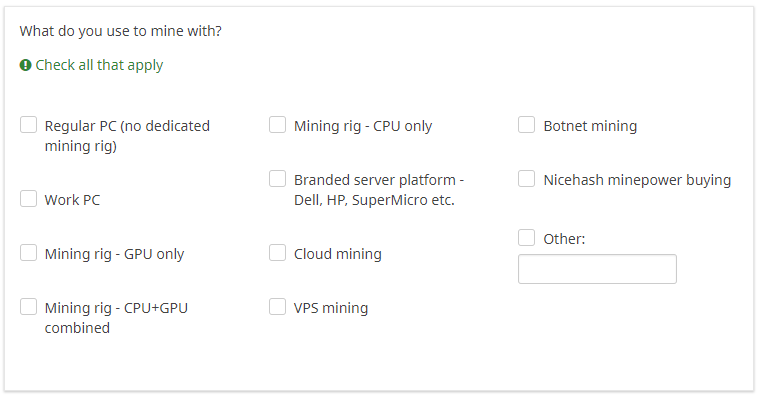
\includegraphics[trim={0.5cm 1.7cm 0.5cm 0.5cm},clip,width=0.9\textwidth]{Screenshot_31.png}
    \caption{Mining setup question.}
    \label{pic:miningquestion}
\end{center}
    \end{figure}
    
    \end{frame}
    \begin{frame}{Výsledky | Ukázka z nasbíraných dat}
    \begin{center}
\begin{figure}[H]
\begin{tikzpicture}
\begin{axis}[
    xbar stacked,
    y dir = reverse,
    legend style={
    legend columns=2,
        at={(xticklabel cs:0.5)},
        anchor=north,
        draw=none
    },
    ytick=data,
    axis y line*=none,
    axis x line*=bottom, %bottom
    tick label style={font=\footnotesize},
    legend style={font=\footnotesize,fill=black,draw=white},
    label style={font=\footnotesize},
    xtick={0,100},
    width=.74\textwidth,
    bar width=6mm,
    xlabel={Time in ms},
    yticklabels={ Default Windows Updates, Activated Windows, Update delay, Remote management, Windows Firewall, Automation tools, Automatic deploy},%yticklabels={ Default Windows Updates, Activated Windows, Update delay, iGPU bug, AV software, Windows Deffender, Remote mgmt, Windows Firewall, Automation tools, Automatic deploy},
    xmin=0,
    xmax=100,
    area legend,
    xticklabel={\pgfmathparse{\tick}\pgfmathprintnumber{\pgfmathresult}\%},
    y=8mm,
    enlarge y limits={abs=0.625},
]
\addplot[1,fill=1] coordinates {(25,1) (54,2) (59,3)  (31,4) (36,5) (56,6) (28,7)};
%{(113,0) }; absolutni cisla, potrebuje to procenta
\addplot[4,fill=4] coordinates { (75,1) (46,2) (41,3) (69,4) (64,5) (44,6) (72,7)};
%\addplot[1,fill=1] coordinates {(25,1) (54,2) (59,3) (8,4) (21,5) (44,6) (31,7) (36,8) (56,9) (28,10)};
%{(113,0) }; absolutni cisla, potrebuje to procenta
%\addplot[4,fill=4] coordinates { (75,1) (46,2) (41,3) (92,4) (79,5) (56,6) (69,7) (64,8) (44,9) (72,10)};
\legend{Yes, No
}
\coordinate (A) at (15,0);% ******** start of changes ************
\coordinate (B) at (70,0);
\coordinate (C) at (40,-8mm);% ******** start of changes ************
\coordinate (D) at (70,-8mm);
\coordinate (E) at (40,-16mm);% ******** start of changes ************
\coordinate (F) at (70,-16mm);
\coordinate (G) at (15,-24mm);% ******** start of changes ************
\coordinate (H) at (70,-24mm);
\coordinate (I) at (15,-32mm);% ******** start of changes ************
\coordinate (J) at (70,-32mm);
\coordinate (K) at (40,-40mm);% ******** start of changes ************
\coordinate (L) at (70,-40mm);
\coordinate (M) at (15,-48mm);% ******** start of changes ************
\coordinate (N) at (70,-48mm);
\end{axis}  
\node at (A) {10};
\node at (B) {29};% ********* end of changes **********
\node at (C) {21};
\node at (D) {18};% ********* end of changes **********
\node at (E) {23};
\node at (F) {16};% ********* end of changes ********** 
\node at (G) {14};
\node at (H) {25};% ********* end of changes **********   
\node at (I) {24};
\node at (J) {15};% ********* end of changes **********
\node at (K) {22};
\node at (L) {17};% ********* end of changes **********
\node at (M) {11};
\node at (N) {28};% ********* end of changes **********
\end{tikzpicture}
\caption{Windows mining setup preferences.}
\label{chart:windowshabits}\end{figure}\end{center}

    \end{frame}
    \subsection{Automatizace}
    \begin{frame}{Automatizace}
    
    \begin{multicols}{2}
OS: Linux
\begin{itemize}
\item Kickstart instalace
\item Spuštění Ansible playbooku
\item Node připraven k těžbě
\end{itemize}
Statistiky:
\begin{itemize}
\item Instalace OS - 5 minut
\item Ansible (aktualizace OS, instalace XMR stak, začátek těžby) - 6 minut
\end{itemize}

\columnbreak
OS: Windows
\begin{itemize}
\item Autounattend instalace
\item Spuštění Ansible playbooku
\item Node připraven k těžbě
\end{itemize}
Statistiky:
\begin{itemize}
\item Instalace OS - 11 minut
\item Ansible (aktualizace OS, instalace XMR stak, začátek těžby) - 46 minut
\end{itemize}
\end{multicols}
Primárně testováno na i5-4460, SSD sestavě. Podobných výsledků bylo dosaženo i na Dell PowerEdge R610 a R210 testovacích serverech (rozdíl v boot time kvůli serverové desce).
 
 
 \tikz[remember picture,overlay] \node[opacity=0.8,inner sep=10pt] at ($(current page.45)+(0,-1.4)$)
 {
\includegraphics[width=0.25\textwidth]{ansible-redhat.png}};

%     \begin{figure}
%  \centering
%  
\includegraphics[width=0.3\textwidth]{ansible-redhat.png}
%  \caption{Monero Github \& Reddit.}  \label{fig:xray}
%\end{figure}
    \end{frame}
  \end{darkframes}
  
  \AtBeginSection[]{% Print an outline at the beginning of sections
    \begin{frame}<beamer>
      \frametitle{Obsah sekce \thesection}
      \begin{multicols}{2}      
      \tableofcontents[currentsection]
      \end{multicols}
    \end{frame}}
    
  \begin{darkframes}
    \section{Závěr}
    \subsection{Webový portál}
    \begin{frame}{Webový portál}
      	\begin{figure}
  \centering
  
\includegraphics[trim={0 1cm 0 0},clip,width=0.85\textwidth]{ssme-portal.png}
% \caption{Specifické požadavky respondentů.}  \label{fig:xray}
\end{figure}
    \end{frame}
    \subsection{Open-source}
    \begin{frame}{Open-source}
     	\begin{figure}
  \centering
  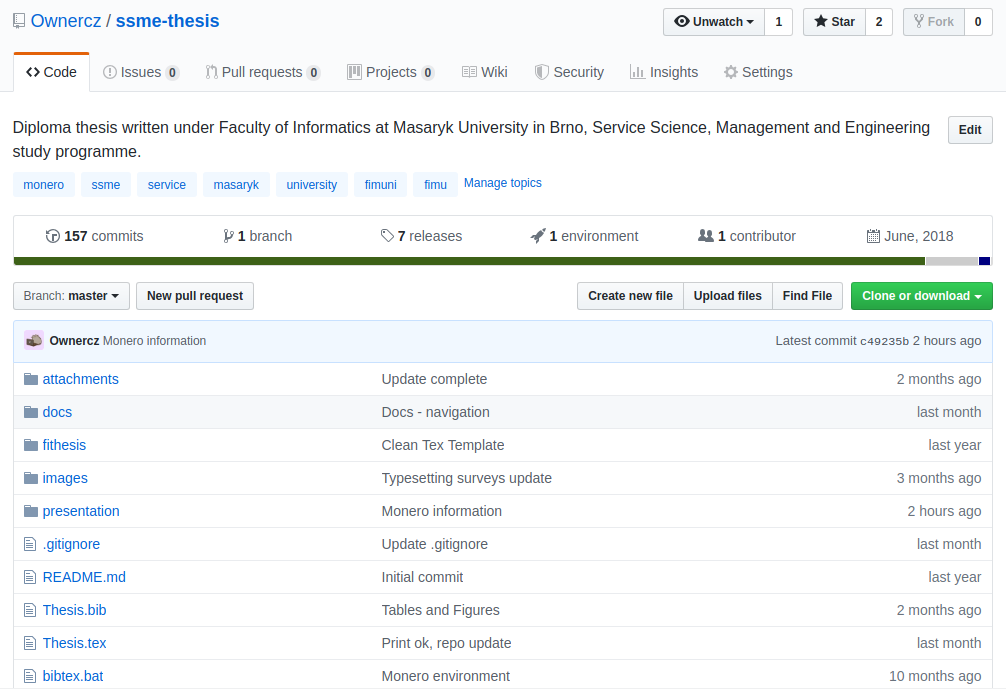
\includegraphics[width=1\textwidth]{github-repo.png}
% \caption{Specifické požadavky respondentů.}  \label{fig:xray}
\end{figure}
    \end{frame}
  \end{darkframes}
  
  \begin{frame}{}
\end{frame}
    
  \AtBeginSection[]{% Print an outline at the beginning of sections
    \begin{frame}<beamer>
      \frametitle{Obsah sekce \thesection}
      \begin{multicols}{2}      
      \tableofcontents[currentsection]
      \end{multicols}
    \end{frame}}
    
  \begin{darkframes}
    \section{Reakce na posudky, dotazy}
     \begin{frame}{Installation videos}
     	\begin{figure}
\say{I appreciate multiple appendices with the data and the
complete questionnaires, as well as the videos of the installation process (although the Linux
link in the repository seems to be broken as of 6th June 2019).}
\begin{itemize}
\item Špatně nastavená viditelnost videa (nastaveno soukromé místo publikovaného).
\item Opraveno, při prezentaci jsem vždy ukazoval z notebooku, kde byl přihlášený Google účet.
\end{itemize}
    \end{figure}
    \end{frame}

        \begin{frame}{Monero community feedback}
     \say{ I’d appreciate knowing
from the author what was the reception of the work by the Monero community (if any).}
    \end{frame}
       \begin{frame}{Monero community feedback}
     	\begin{figure}
  \centering
  
\includegraphics[width=0.68\textwidth]{community-facebook.png}
% \caption{Specifické požadavky respondentů.}  \label{fig:xray}
\end{figure}
    \end{frame}    
    \begin{frame}{Monero community feedback}
     	\begin{figure}
  \centering
  
\includegraphics[width=1\textwidth]{community-reddit.png}
% \caption{Specifické požadavky respondentů.}  \label{fig:xray}
\end{figure}
    \end{frame}
        \begin{frame}{Monero community feedback}
     	\begin{figure}
  \centering
  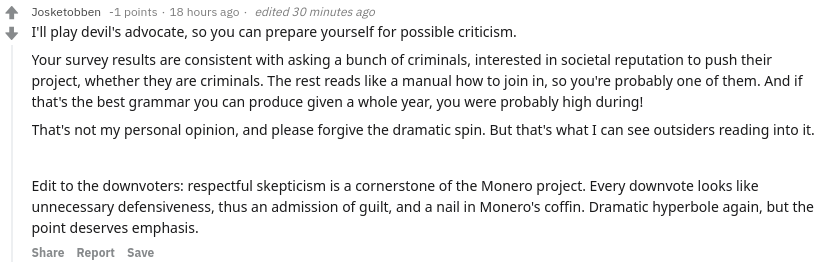
\includegraphics[width=1\textwidth]{community-redditnext.png}
% \caption{Specifické požadavky respondentů.}  \label{fig:xray}
\end{figure}
    \end{frame}
      
    \begin{frame}{Monero community feedback}
     	\begin{figure}
  \centering
  
\includegraphics[width=1\textwidth]{reddit-commentnext.png}
  
\includegraphics[width=0.4\textwidth]{community-redditcomment.png}
% \caption{Specifické požadavky respondentů.}  \label{fig:xray}
\end{figure}
    \end{frame}
    
        \begin{frame}{Ansible}
     \say{On the other hand, I appreciate the
effort of having the automation setup available for both Linux and Windows (making it must
have required different sets of skills). Customization possibilities of the Ansible playbooks are
not mentioned much (Are there any?).}
	\begin{itemize}
	\item Každá rolí obsahuje složku defaults, ve které existuje \texttt{main.yml} s proměnnými pro úpravu.
	\begin{itemize}
	\item U \texttt{ansible-win-apps} tak může uživatel změnit adresu peněženky, pool, konfiguraci webového rozhraní a další věci týkající se těžebního software.
	\end{itemize}
	\end{itemize}
    \end{frame}


        \begin{frame}{Bias}
     \begin{small}
     \say{Secondly, you do not consider the social desirability bias much – people
will not readily admit illegal activity (and drug buying, darknet transactions, ...). I appreciate
the data cleaning, but could that not have introduced/increased the bias?}
     \end{small}

Plně souhlasím, vypadá to zvláštně, když odfiltruji \say{Partially answered or unanswered questionnaires were not taken into account (261 out of 323).} \textbf{Měl jsem dodat popis metodiky, co je částečně nebo vůbec.}
\begin{itemize}
\item Částečné nebo vůbec = počet vyplněných otázek z celku < 5. 
\item Skutečnost: 261 odfiltrovaných = buď žádná odpověď nikde nebo náhodné zakliknutí jedné otázky.
\end{itemize}
    \end{frame}
        \begin{frame}{Mining setup vs questionnaire}
     \say{Moreover, I miss how precisely these
build on the results from the questionnaire in chapter 5. Similarly so for the designed mining
setup automation in chapter 9 (How does it build on the questionnaire results? What would
you have done differently without the questionnaire?). }
\begin{itemize}
\item Získání informací o tom, jaký software pro těžbu se používá [XMR-Stak/XMRig/Wallet?].
\item Zda má cenu dělat návod na mining operation (nepoužívají pronajatý výkon, cloud?)
\item Na jakých platformách se těží? (Windows = jednodušší a lépe optimalizované z hlediska paměti a GPU)
\end{itemize}

    \end{frame}

        \begin{frame}{Userbase/minerbase}
     \say{The sample may not be representative of the Monero
userbase/minerbase at all. Can we at least make a comparison to some general Monero stats?
How many users/wallets are there? What countries seem Monero users to dominantly be
from? (At least an estimate based on the forums, etc.) Could your sample mislead the results?
In what way precisely?}
    \end{frame}
    
        \begin{frame}{Userbase/minerbase}
     \say{The sample may not be representative of the Monero
userbase/minerbase at all. Can we at least make a comparison to some general Monero stats?}
\begin{itemize}
\item Přímo uživatelů - vzhledem k principu fungování Monera reprezentativně ne.
\item Z fór, Redditu, Facebooku - vždy to bude omezená množina (podobně jako u mých dat).
\begin{itemize}
\item Scrapováním těchto zdrojů by šlo docílit podrobnějších informací.
\end{itemize}
\item \say{Nejreprezentativnějším} údajem = rozdělení hashrate do poolů a princip, že většina lidí chce těžit tam, kam mají nejnižší latenci (problém - co když neexistuje v dané lokalitě atraktivní pool).
\end{itemize}
    \end{frame}
    
            \begin{frame}{Userbase/minerbase}
     \say{What countries seem Monero users to dominantly be
from? (At least an estimate based on the forums, etc.) Could your sample mislead the results?
In what way precisely?}
\begin{itemize}
\item Opravdu velký odhad podložený subjektivním pozorováním dle aktivity (čas postování, komentáře) - USA.
\item Použitý vzorek mohl ovlivnit výsledky například v:
\begin{itemize}
\item Způsob užití měny (dle geo/socio/ekonomických podmínek)
\item Použitý hardware a software klientů (preference určitého OS apod.)
\item Výběr těžebního poolu (dle lokality)
\end{itemize}
\end{itemize}
    \end{frame}
    

    \begin{frame}{Research questions}
      \say{\begin{small}
      What parts of the
study address what research questions? What are the conclusions regarding the individual
questions?).
      \end{small}}
       \begin{multicols}{2}
       Research questions
      \begin{small}
      \begin{enumerate}
      \item What are Monero’s main use cases? How do participants
perceive Monero’s features?
      \item What are participant’s ways of wallet access and storage?
      \item What security incidents have affected users? How did they
deal with them?
      \item In case of recovery, how did they recover their keys?
      \end{enumerate}
      Pairing in text
      \begin{enumerate}
            \item Chapter 5.4.2 Monero usage, Table 5.1/5.2, Figure 5.9
      \item Chapter 5.4.1 and 5.4.3 Monero key and coin management, Figure 5.11, 5.4-7 
      \item Chapter 5.4.4 and 5.4.5 Monero recovery/malicious software
      \item Chapter 5.4.4, Figure 5.12, 5.13
      \end{enumerate}
      \end{small}
      \end{multicols}
    \end{frame}
    
        \begin{frame}{Survey Methodology}
     \say{However, I see some deficiencies in survey methodology: Where did the
answer options to the individual questions come from? E.g. is there really a difference in
the answers for profit and as an investment?). }
\begin{itemize}
\item Tyto možnosti, jak odpovědět, byly vytvořeny mnou na základě toho, za co se může kromě Monera i jiný druh měny použít. Obecné kategorie + přidány specifické věci, pro které by mohlo být Monero použito (gambling, illegal use cases).
\end{itemize}
\end{frame}

\begin{frame}{Survey Methodology - pokračování}

\say{Furthermore, I miss the options indicating the
participant does not know or thinks the question does not apply to them (details why this may
be a problem described later).}

\begin{itemize}
\item Problém - rozdílnost online formuláře vs jeho export v PDF verzi pro tisk diplomové práce.
\item Reálně tuto možnost měli viz další slidy.
\end{itemize}
    \end{frame}
        \begin{frame}{Survey Methodology - pokračování}
     	\begin{figure}
  \centering
  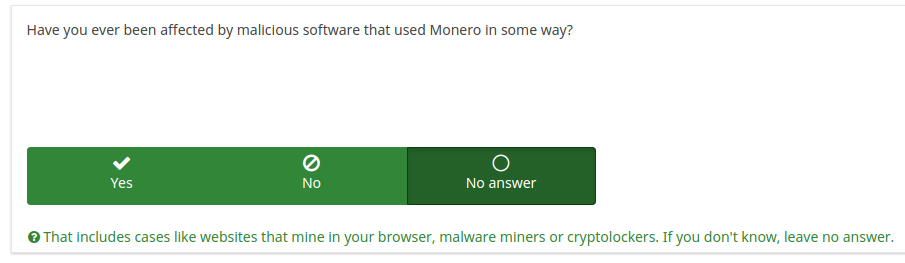
\includegraphics[width=1\textwidth]{survey-answer.png}
% \caption{Specifické požadavky respondentů.}  \label{fig:xray}
\end{figure}
    \end{frame}
            \begin{frame}{Survey Methodology - pokračování}
     	\begin{figure}
  \centering
  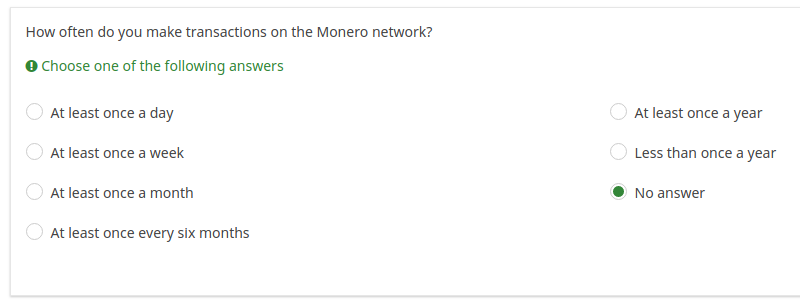
\includegraphics[width=1\textwidth]{survey-answernext.png}
% \caption{Specifické požadavky respondentů.}  \label{fig:xray}
\end{figure}
    \end{frame}
            \begin{frame}{Survey Methodology - pokračování}
     	\begin{figure}
  \centering
  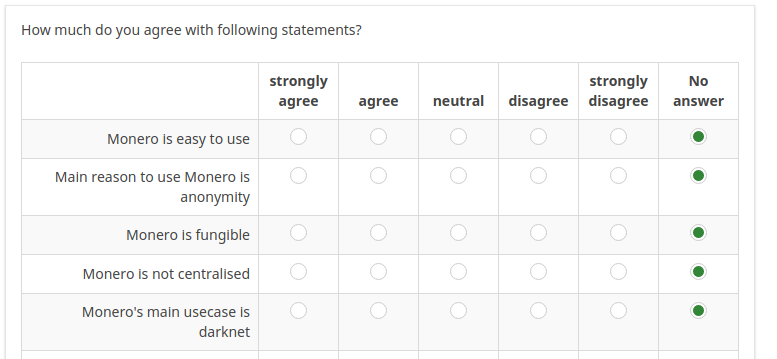
\includegraphics[width=1\textwidth]{survey-answernextanother.png}
% \caption{Specifické požadavky respondentů.}  \label{fig:xray}
\end{figure}
    \end{frame}

    



  \end{darkframes}

\end{document}
